\documentclass[UTF8]{ctexart}
\usepackage{amsmath}
\usepackage{graphicx}
\usepackage{hyperref}
\usepackage{tabularx}
\usepackage{booktabs}
\usepackage{geometry}
\geometry{a4paper, margin=1in}

\title{Modbus RTU Learning based on RS485}
\author{倪煜晖}
\date{\today}

\begin{document}

\maketitle

% 生成目录
\tableofcontents

\section{说明}
记录Modbus RTU通讯协议学习过程,用于实现xArm6机械臂与知行机器人夹爪之间的通信,以备后续查看使用。

\section{Modbus RTU与 RS485初探}

\subsection{简介}
Modbus是一种应用协议,RTU是一种通信模式,而RS485是总线串行标准。前二者工作在应用层与链路层,而RS485工作在物理层。

\subsection{联系与区别}
\begin{itemize}
    \item Modbus RTU:一种主从通信协议。它定义了数据传输的规则,包括数据帧的格式、帧的开始和结束标志、地址域、功能码、数据区和错误检测域等。例如,在一个 Modbus RTU 帧中,地址域用于标识从设备的地址,功能码用于指定主设备希望从设备执行的操作,如读取寄存器、写入寄存器等。
    \item RS485:一种电气接口标准,它规定了数据传输的物理层特性,如信号电平、传输速率、传输距离等。RS - 485 支持多点通信,能够在长距离和高噪声环境下可靠地传输数据。
\end{itemize}

在我们的任务中,RS - 485 提供了硬件层面的通信通道,Modbus RTU 则是在这个通道上运行的协议,规定了数据的传输格式、帧结构等内容,二者相互配合来实现设备之间的通信。

\subsection{重点}
RS485使用差分传输模式,使用双绞线$A,B$之间的电位差来实现通信。它的核心是一个主机与多个从机的通讯。这里需要注意的是,这和$\textbf{I/O}$通信完全没有关系,也就是说,我们$\textbf{I/O}$的五根线大概是没用的。由于RS485协议对电位敏感,建议在之后断开对这五根线的连接,保证接地唯一。


% 插入图片示例
\begin{figure}[htbp]
    \centering
    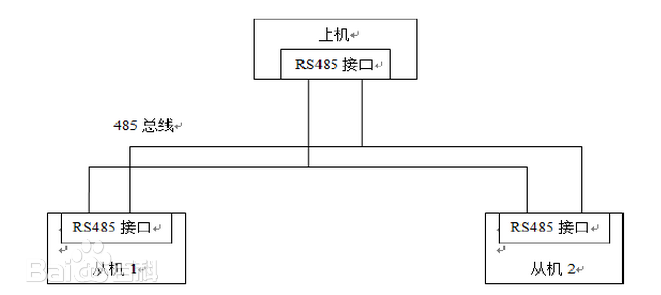
\includegraphics[width=0.8\textwidth]{master_slave.png}
    \caption{一主多从}
    \label{ms}
\end{figure}
确认接线之后,我们把注意力更多放在Modbus RTU上。


\section{使用机器码实现Modbus RTU通信}
\subsection{参数配置}
\subsubsection{夹爪要求}
\begin{itemize}
    \item 波特率: 115200
    \item ID: 默认为1
    \item 数据格式:默认的数据格式为无检验
    \item 校验模式:使用16进制CRC校验码,低字节在前
\end{itemize}

这里highlight校验模式。

使用手册中给出了示例通信码 01 06 01 02 00 64 28 1D。
具体解释会在后面章节注明,也可以直接参照表格\eqref{tab:data_frame}。注意到,这里的最后两位是校验码,由前六位决定。我们遇到的报文无效问题由一部分应该是这个原因。


\begin{table}[htbp]
    \centering
    \caption{数据帧格式说明}
    \label{tab:data_frame}
    \begin{tabularx}{\textwidth}{>{\raggedright\arraybackslash}p{0.15\textwidth} 
                                >{\raggedright\arraybackslash}p{0.1\textwidth} 
                                >{\raggedright\arraybackslash}X 
                                >{\raggedright\arraybackslash}X}
        \toprule
        \textbf{数据} & \textbf{字节} & \textbf{数据说明} & \textbf{备注} \\ 
        \midrule
        01            & 1             & 从机地址           & 0x01 为设备 ID 号,0x00 为广播地址(无回应) \\ 
        \midrule
        06            & 1             & 功能码             & 单个保持寄存器的写入 \\ 
        \midrule
        01 02         & 2             & 数据地址           & 0x0102 为需要执行功能码的数据地址(执行器临时区运动位置) \\ 
        \midrule
        00 64         & 2             & 数据值             & 0x0064 为 16 进制的 100,即将执行器运动位置(临时区)的值设定为 100 \\ 
        \midrule
        28 1D         & 2             & CRC 校验码         & 16 进制 CRC 校验码,低字节在前 \\ 
        \bottomrule
    \end{tabularx}
\end{table}

为了生成正确的校验码,我找到了\href{http://www.ip33.com/crc.html}{生成网站}并且正确生成了校验码。

\begin{figure}[htbp]
    \centering
    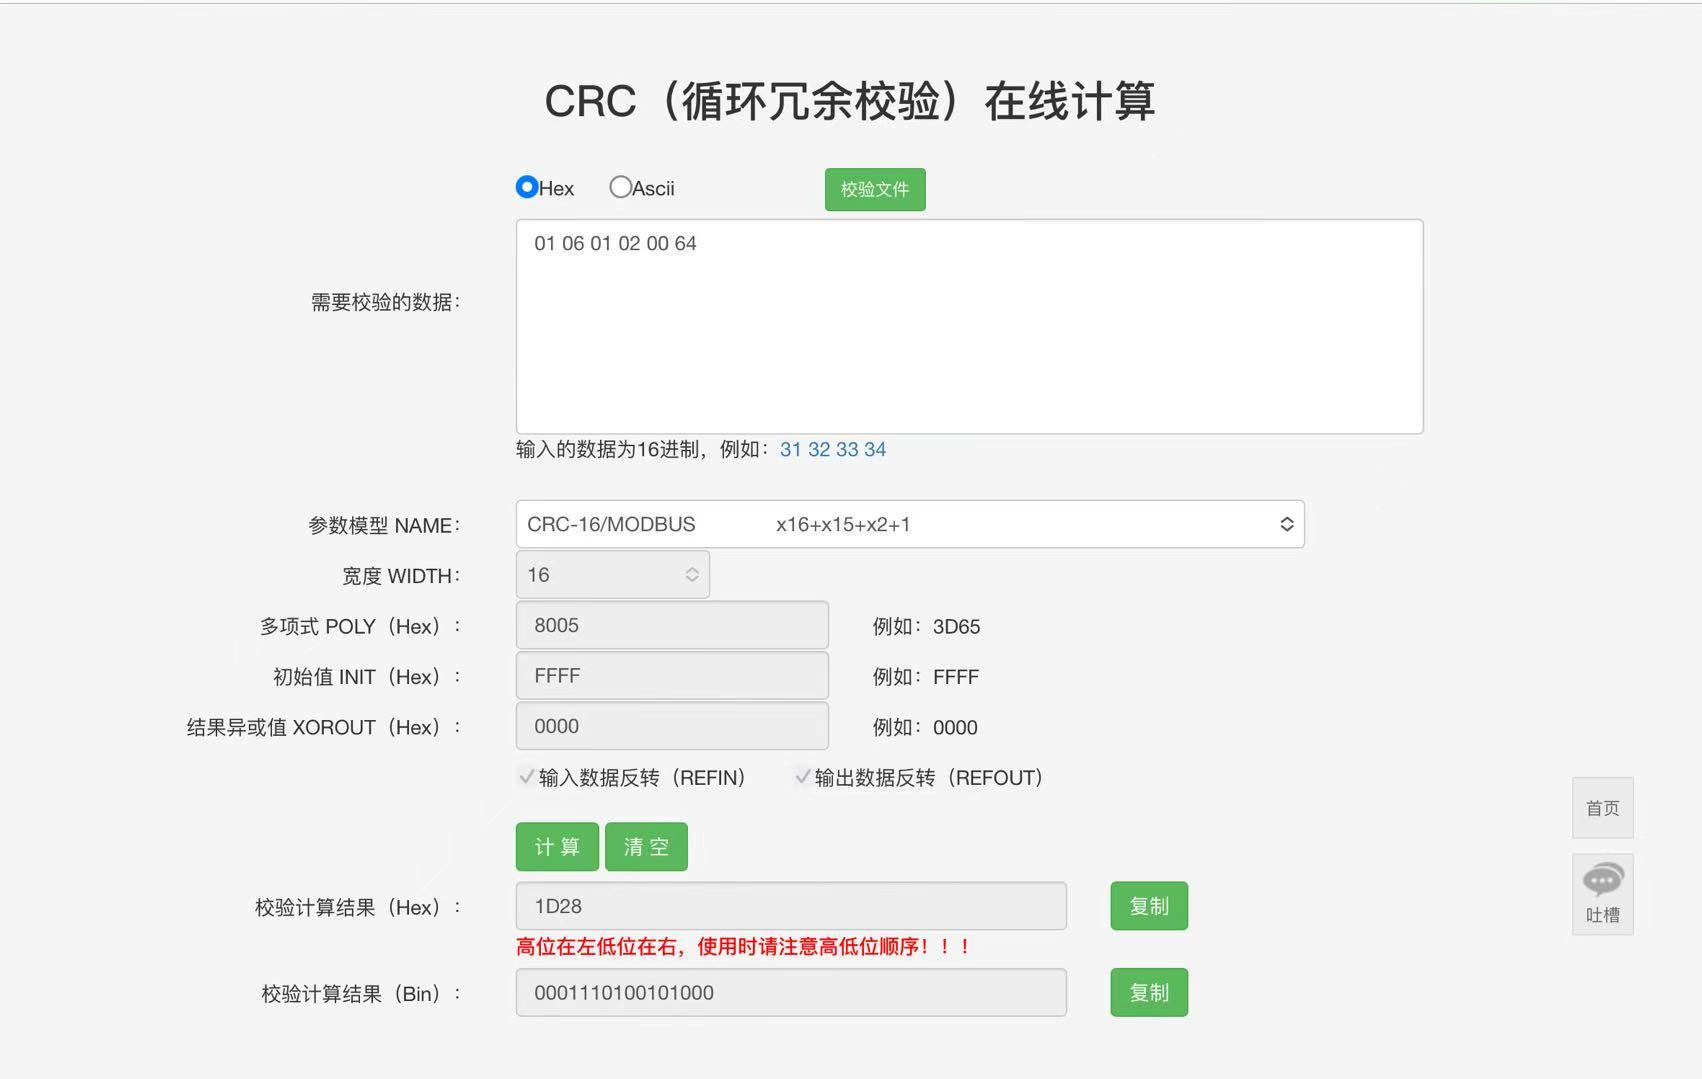
\includegraphics[width=0.8\textwidth]{ip33.jpg}
    \caption{校验码}
    \label{verti}
\end{figure}

值得注意的是,xArm手册中提到自动生成CRC校验码,不知道使用的是否为16位,也不知道采用的是低位在前还是高位在前,可能成为核心问题。

\subsubsection{xArm要求}
\begin{itemize}
    \item 波特率:默认200000
    \item 12位6字节十六进制编码,\bf{自动生成}CRC校验码
\end{itemize}

之前一直无法执行很有可能是位数不对与设备ID不对,应当只输入6字节,选定正确设备ID也就是1,后续尝试。

\subsection{通用Modbus RTU指令(TO DO)}
TO DO
\subsection{夹爪执行器特有参数(TO DO)}
TO DO
\section{使用Python调用Modbus RTU(TO DO)}
TO DO

\section{可能的替代方案——I/O控制(TO DO)}
TO DO


\end{document}